
\documentclass[5pt,a4paper]{article}
\usepackage{geometry}
\geometry{
	a4paper,
	total={170mm,257mm},
	left=20mm,
	top=20mm,
}
\usepackage[latin1]{inputenc}
\usepackage{amsmath}
\usepackage{amsfonts}
\usepackage{amssymb}
\usepackage{graphicx}
\usepackage{subfig}
\begin{document}
	\title{Machine learning Homework- Soft-Margin SVM and Kernels }
	\author{Abinav Ravi Venkatakrishnan - 03694216 and Abhijeet Parida - 03679676}
	\maketitle
	\section*{Problem 1:}
	No it will not be the correct label. The training sample depends on the distance from the hyperplane decision boundary $\xi$. If $ \xi < 1 $ for the training sample it gets classified correctly else it gets mis-classified.
	
	\section*{Problem 2:}
	The cost function for soft-margin SVM is 
	\begin{equation}
	min f_0(\textbf{w},b,\xi) = \frac{1}{2}\textbf{w}^T \textbf{w}+ C \sum_{i=1}^{N} \xi_i
	\end{equation}
	C is a penalizing factor on $ \xi $. \\
	case 1: when C = 0 there is no restriction on $\xi$ values.\\
	case 2: when C < 0 it encourages higher values of $\xi$ and hence encouraging mis-classification.  
	\section*{Problem 3:}
	\begin{figure}[!h]%
		\centering
		\subfloat[]
		{{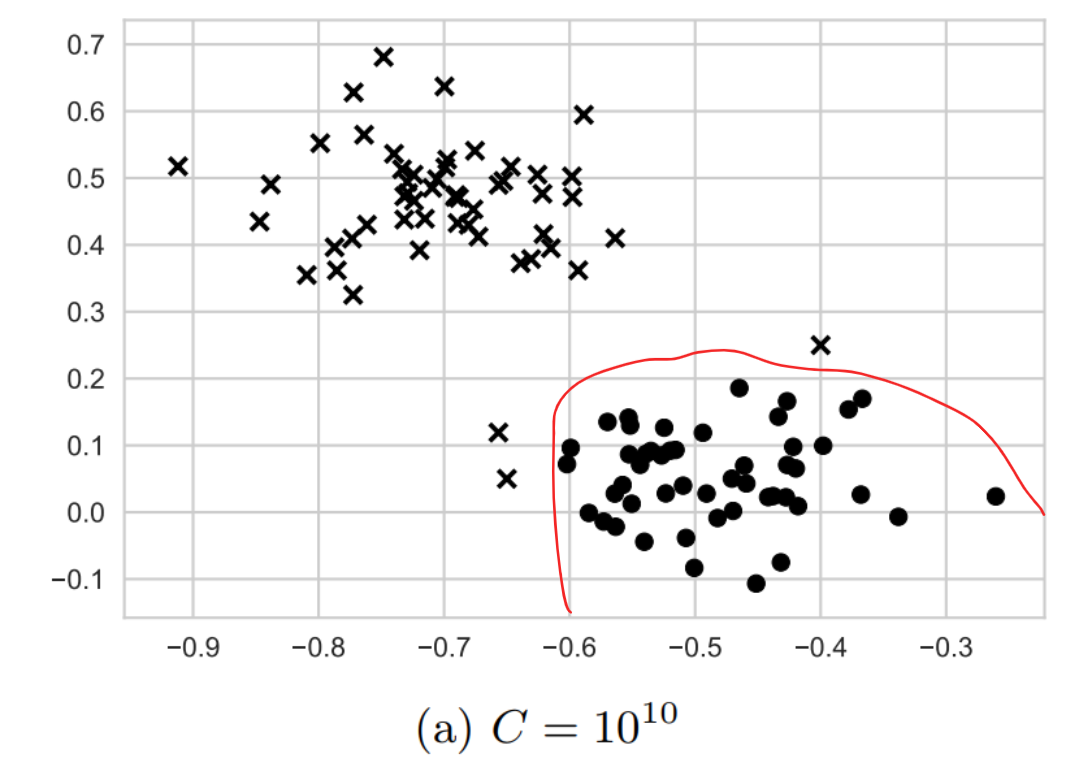
\includegraphics[width=6cm,height=4.5cm]{img1_f.png} }}%
		\qquad
		\subfloat[]
		{{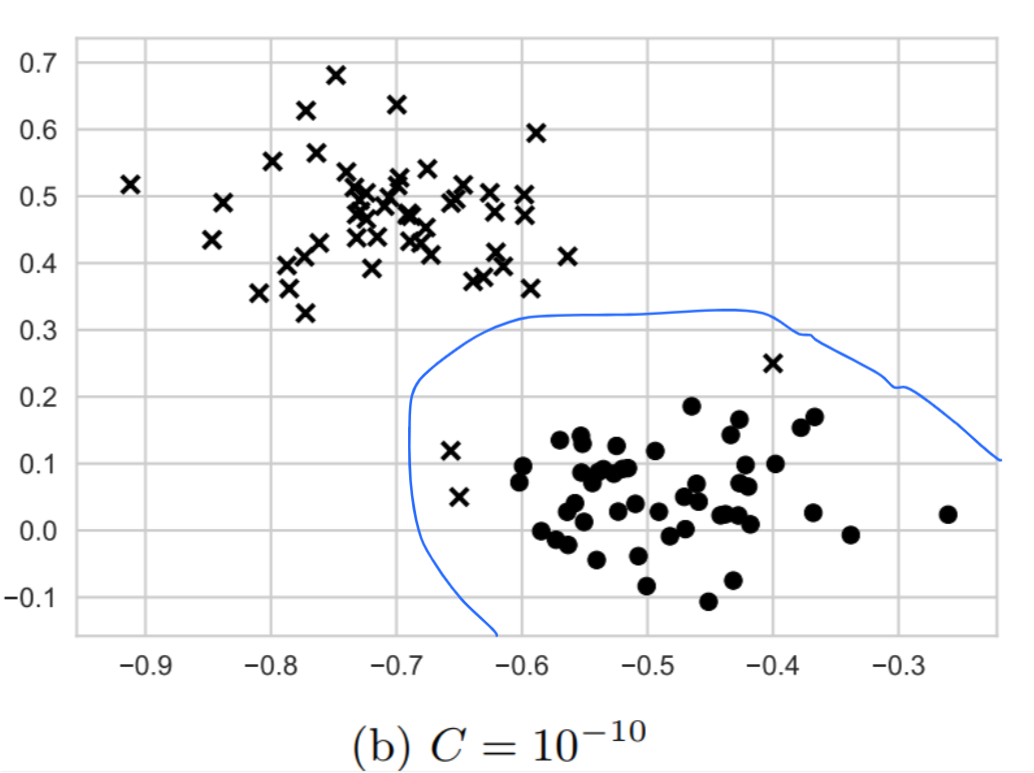
\includegraphics[width=6cm,height=4.5cm]{img2_f.png} }}%
		\caption{}%
	\end{figure}

The first case tends to have hard margin of SVM since the C value is very big and C tends to $\infty$. The second figure on the right has soft margin since the C value is very less and this can take some mis-classification.\\ 
	
	\section*{Problem 4:}
	We know that $ \sum_{i=0}^{N} a_i({x_i}^T {x_j})^i $ is a polynomial kernel. by the kernel preserving operation we know that sum of valid kernel is also a valid kernel and hence $k(x1,x2)$
	
	
	\section*{Problem 6:}
	a) The algorithm is trying to find the matching characters in the given string.\\
	b) The alphabets are mapped from SxS space to real space. The real number is actually a mapping of s$ \ge$0 which means that the Mercer Matrix has values which are positive or zero i.e. the matrix is Positive semi-definite thereby making the Kernel valid. 
	\section*{Problem 7:}
	For linearly separated points the SVM is given by 
	\begin{equation}
	y_i(w^T \phi(x_i)+b) > 0 
	\end{equation} this equation is transformed into a different forms by using the kernel trick for non linear separations. But this is possible when the limit of $\sigma$ tends to zero or very low values of $\sigma$
	
	
\end{document}